% This file was created with tikzplotlib v0.9.12.
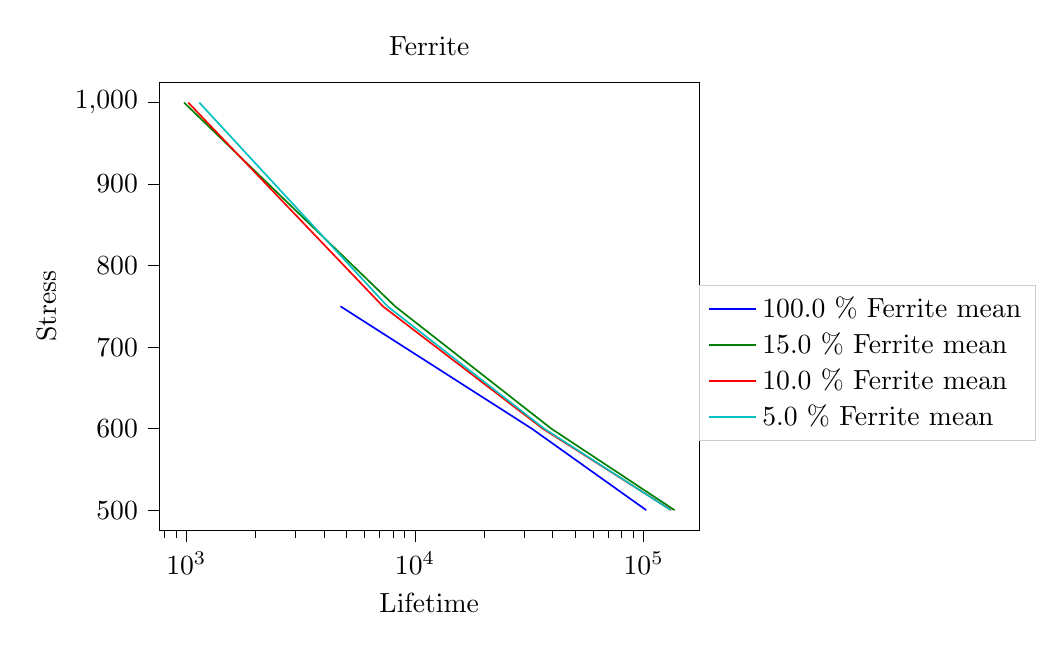
\begin{tikzpicture}

\definecolor{color0}{rgb}{0,0.75,0.75}

\begin{axis}[
legend cell align={left},
legend style={
  fill opacity=0.8,
  draw opacity=1,
  text opacity=1,
  at={(1,0.2)},
  anchor=south west,
  draw=white!80!black
},
log basis x={10},
tick align=outside,
tick pos=left,
title={Ferrite},
x grid style={white!69.0196078431373!black},
xlabel={Lifetime},
xmin=762.921177526063, xmax=174782.525072432,
xmode=log,
xtick style={color=black},
y grid style={white!69.0196078431373!black},
ylabel={Stress},
ymin=475, ymax=1025,
ytick style={color=black}
]
\addplot [semithick, blue]
table {%
102622.170334593 500
32404.8001413774 600
4722.98589714715 750
nan 1000
};
\addlegendentry{100.0 \% Ferrite mean}
\addplot [semithick, green!50!black]
table {%
136528.855124647 500
39445.4435945436 600
8183.13975467324 750
976.682106632312 1000
};
\addlegendentry{15.0 \% Ferrite mean}
\addplot [semithick, red]
table {%
132002.808742684 500
36199.0318401257 600
7240.77939431601 750
1019.53871162753 1000
};
\addlegendentry{10.0 \% Ferrite mean}
\addplot [semithick, color0]
table {%
131464.248344587 500
36727.8351009599 600
7583.9793048352 750
1139.41747782028 1000
};
\addlegendentry{5.0 \% Ferrite mean}
\end{axis}

\end{tikzpicture}
